%% BrainHybridNet -- manuscript for IEEE Journal of Biomedical and Health Informatics (J-BHI)
%% Template: IEEEtran (journal mode), two columns. Compile on Overleaf (IEEEtran is built in).
%% J-BHI: abstract <= 250 words with no abbreviations; 14 pages max incl. supplementary;
%% pages 9-10 cost $250 each and page 11+ $350 each (EMBS author page, checked 2026-10-25).
%% This version is condensed to stay near 8 pages.
%%
%% STATUS: NOT SUBMITTABLE YET. Every \tbd{} marks a number that must come from experiments.

\documentclass[journal]{IEEEtran}

\usepackage{cite}
\usepackage{amsmath,amssymb,amsfonts}
\usepackage{graphicx}
\usepackage{booktabs}
\usepackage{xcolor}
\usepackage{url}

\newcommand{\tbd}[1][]{\textcolor{red}{\textbf{[TBD#1]}}}

\begin{document}

\title{BrainHybridNet: A Lightweight Hybrid CNN--Transformer for Joint Brain Tumor Segmentation, Detection and Grading with Self-Supervised Pre-training and Uncertainty Estimation}

\author{Debobrato~Biswas,~\IEEEmembership{\tbd[: IEEE membership or remove]},
\tbd[: co-author names]
\thanks{Manuscript received \tbd; revised \tbd.}
\thanks{D. Biswas is with the Department of Computer Science and Engineering, Daffodil International University, Dhaka, Bangladesh (e-mail: \tbd[: institutional e-mail]).}
\thanks{\tbd[: co-author affiliations].}}

\markboth{IEEE Journal of Biomedical and Health Informatics}{Biswas \MakeLowercase{\textit{et al.}}: BrainHybridNet}

\maketitle

%% No abbreviations allowed in the J-BHI abstract.
\begin{abstract}
Objective: Automated brain tumor analysis from magnetic resonance images usually requires separate models for segmentation, detection and grading, and most report no measure of confidence. We present a single lightweight model that performs all three tasks and estimates its own uncertainty. Methods: The proposed network combines a two-stage convolutional stem, which preserves high-resolution detail, with a four-layer transformer that models long-range volumetric context. In one forward pass it segments the whole tumor, tumor core and enhancing tumor, detects tumor presence and predicts low- versus high-grade glioma. The encoder is pre-trained by reconstructing masked regions of unlabeled scans; repeated stochastic inference with dropout yields a voxel-wise uncertainty map, and transformer attention provides spatial explanations. Five established networks were re-trained on identical patient-level splits of the 2021 Brain Tumor Segmentation challenge data (1,251 patients) for comparison. Results: On the held-out test set the model reaches Dice scores of \tbd{}, \tbd{} and \tbd{} for whole tumor, tumor core and enhancing tumor, with \tbd{} million parameters and \tbd{} milliseconds per volume crop; \tbd[: grading area under the curve, calibration error and external-validation result]. Conclusion: \tbd[: measured trade-off between accuracy, model size and calibration]. Significance: A compact model that segments, detects and grades brain tumors while flagging uncertain regions can support radiologist review on standard clinical hardware.
\end{abstract}

\begin{IEEEkeywords}
Brain tumor segmentation, glioma grading, magnetic resonance imaging, masked image modeling, transformer, uncertainty estimation.
\end{IEEEkeywords}

\section{Introduction}
\IEEEPARstart{G}{lioblastoma} (WHO grade 4) has a median overall survival of 14.6 months under standard treatment~\cite{stupp2005}, and about 308,000 new brain and central nervous system tumors were estimated worldwide in 2020~\cite{sung2021globocan}. Delineating the whole tumor (WT), tumor core (TC) and enhancing tumor (ET) on multi-modal MRI (T1, contrast-enhanced T1ce, T2, FLAIR)~\cite{gordillo2013} guides surgery, radiotherapy and response assessment, but manual delineation is slow and raters agree only to Dice 0.74--0.85~\cite{menze2015}.

CNNs such as 3D U-Net~\cite{ronneberger2015,cicek2016} capture local structure but not long-range context; transformers~\cite{vaswani2017,dosovitskiy2021} do, at high data and compute cost. Hybrid designs~\cite{chen2021transunet,wang2021transbts,wu2023dformer} combine both, but most solve one task, give point predictions only~\cite{gal2016} and have tens of millions of parameters~\cite{ker2018}.

We propose BrainHybridNet. Our contributions are:
\begin{itemize}
\item a lightweight hybrid encoder (CNN stem with high-resolution skips, four-layer transformer bottleneck) with \tbd{} million parameters;
\item 3D masked image modeling applied before the CNN stem of a hybrid encoder, extending ViT self pre-training on target data~\cite{zhou2023selfmae}, with measured effects on accuracy and label efficiency;
\item joint segmentation, detection and LGG/HGG grading in one pass;
\item Monte Carlo dropout uncertainty, evaluated for calibration and correlation with error, and attention maps evaluated against reference masks;
\item a reproducible comparison with five re-trained baselines on identical splits, with confidence intervals, paired tests and external validation; code, splits and weights are public.
\end{itemize}

\section{Related Work}
\textit{Segmentation networks.} 3D U-Net~\cite{cicek2016}, SegResNet~\cite{myronenko2019} and the self-configuring nnU-Net~\cite{isensee2021nnunet} are strong CNN baselines. UNETR~\cite{hatamizadeh2022unetr} and SwinUNETR~\cite{tang2022swinunetr,liu2021swin} use transformer encoders; TransBTS~\cite{wang2021transbts}, MedT~\cite{valanarasu2021medt}, UCTransNet~\cite{wang2022uctransnet} and D-Former~\cite{wu2023dformer} mix convolution and attention.
\textit{Self-supervised learning.} Contrastive learning~\cite{chen2020simclr,caron2021dino,sowrirajan2021mococxr} and masked image modeling~\cite{he2022mae,xie2022simmim} reduce label needs; MAE self pre-training improves BraTS segmentation~\cite{zhou2023selfmae}.
\textit{Uncertainty.} Bayesian networks~\cite{neal1996}, deep ensembles~\cite{lakshminarayanan2017} and Monte Carlo dropout~\cite{gal2016} estimate epistemic uncertainty; in neuroimaging it has been linked to errors~\cite{nair2020} and used for quality control~\cite{roy2018}.
\textit{Grading.} WHO CNS5 grading uses histology and molecular markers~\cite{louis2021who}; imaging-based grading uses radiomics~\cite{zhou2018radiomics} or CNNs~\cite{chang2018idh}, usually separate from segmentation.

\section{Method}

\begin{figure*}[!t]
\centering
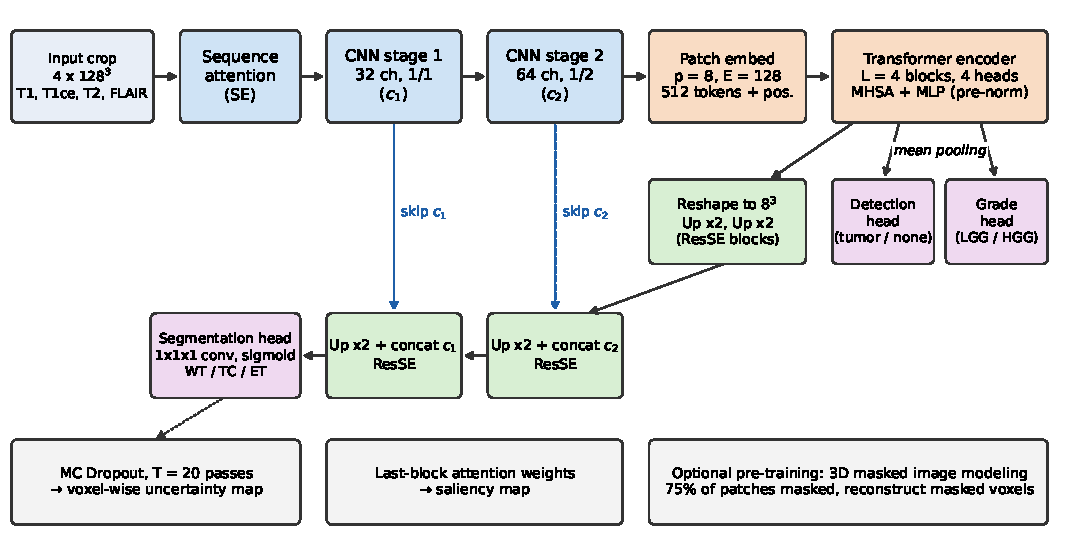
\includegraphics[width=0.92\textwidth]{figures/fig1_architecture.pdf}
\caption{BrainHybridNet. Sequence attention and a two-stage CNN stem give skip features $c_1$, $c_2$; 512 tokens from $8^3$ patches of $c_2$ pass four transformer blocks. Pooled tokens feed detection and grade heads; the decoder fuses $c_2$ and $c_1$ before the WT/TC/ET head. Monte Carlo dropout gives uncertainty, last-block attention a saliency map.}
\label{fig:arch}
\end{figure*}

\subsection{Architecture}
Fig.~\ref{fig:arch} shows the network. Input $\mathbf{X}\in\mathbb{R}^{B\times4\times D\times H\times W}$ (four z-scored sequences, $128^3$ crops) is re-weighted per sequence by squeeze-and-excitation and passed through two stem stages:
$c_1=\mathrm{ReLU}(\mathrm{BN}(\mathrm{Conv}_{3,1}(\mathbf{X})))$ (32 channels, full resolution) and $c_2=\mathrm{ReLU}(\mathrm{BN}(\mathrm{Conv}_{3,2}(c_1)))$ (64 channels, half resolution).
A strided convolution turns $8^3$ patches of $c_2$ into $N=512$ tokens of size $E=128$ with learned positional embeddings $\mathbf{P}$, followed by $L=4$ pre-norm transformer blocks (4 heads, MLP ratio 4, GELU~\cite{hendrycks2016gelu}, dropout 0.1)~\cite{ba2016layernorm}:
\begin{equation}
z'_l=z_l+\mathrm{MHSA}(\mathrm{LN}(z_l)),\quad z_{l+1}=z'_l+\mathrm{MLP}(\mathrm{LN}(z'_l)).
\end{equation}
The decoder reshapes tokens to an $8^3$ grid, applies 3D dropout (0.1), and upsamples four times with transposed convolutions and residual squeeze-and-excitation (ResSE) blocks, concatenating $c_2$ and $c_1$ at matching resolutions. Heads: a $1\times1\times1$ convolution with sigmoids for WT/TC/ET; detection $\mathrm{Linear}(E,128)\!\rightarrow\!\mathrm{ReLU}\!\rightarrow\!\mathrm{Linear}(128,2)$ and grading $\mathrm{Linear}(E,64)\!\rightarrow\!\mathrm{ReLU}\!\rightarrow\!\mathrm{Linear}(64,2)$ on mean-pooled tokens. As BraTS has no tumor-free subjects, detection is trained per crop (positive if $\geq100$ WT voxels); subjects without grade labels are ignored by the grading loss.

\subsection{Masked image modeling}
Following SimMIM~\cite{xie2022simmim} in 3D, 75\% of token positions are masked; their $16^3$ input regions are zeroed before the stem (so nothing leaks through convolutions) and the tokens replaced by a learned mask embedding. A linear head reconstructs the $4\times16^3$ voxels of each masked region; the loss is the mean squared error to per-patch normalized targets over masked patches only. Pre-training uses only the training folds.

\subsection{Uncertainty}
With batch normalization frozen and dropout active~\cite{gal2016}, $T=20$ sliding-window passes give the mean $\mu$ and voxel-wise variance $\sigma^2=\frac{1}{T}\sum_t(\sigma(\hat{Y}^{(t)})-\mu)^2$.

\subsection{Training}
$\mathcal{L}=0.6\,\mathcal{L}_{\mathrm{seg}}+0.2\,\mathcal{L}_{\mathrm{det}}+0.2\,\mathcal{L}_{\mathrm{grade}}$, with cross-entropy for detection and grading and the Tversky loss~\cite{salehi2017tversky} ($\alpha=0.3$, $\beta=0.7$) per region for segmentation. AdamW~\cite{loshchilov2019adamw} (learning rate $10^{-4}$, weight decay $10^{-4}$, clipping 1.0), 10 warm-up epochs then cosine decay~\cite{loshchilov2017sgdr}, 300 epochs (pre-training 100 epochs at $1.5\times10^{-4}$), batch 2, mixed precision; flips, intensity scaling/shift and Gaussian noise; crops centered on tumor with probability 0.66; best mean validation Dice per fold.

\section{Experimental Setup}
\textit{Data.} BraTS 2021~\cite{baid2021brats}: 1,251 subjects, four co-registered skull-stripped sequences at 1\,mm$^3$; WT, TC and ET from the expert labels. A subject-level hold-out test set (15\%, \tbd{} subjects) is used once; the rest forms five folds shared by all models. Grading uses UCSF-PDGM~\cite{calabrese2022ucsfpdgm} (WHO grade), which also serves as an external segmentation test set.
\textit{Baselines.} 3D U-Net, SegResNet, UNETR, SwinUNETR (MONAI~\cite{cardoso2022monai}) and nnU-Net v2, all re-trained on the same folds and preprocessing.
\textit{Metrics.} Dice and HD95 per region (BraTS conventions for empty masks); AUC, balanced accuracy, sensitivity and specificity; voxel-level expected calibration error~\cite{guo2017calibration}; Spearman correlation of case uncertainty with $1-$Dice; parameters, MACs, latency and memory on \tbd[: GPU]. Mean $\pm$ SD, 95\% bootstrap intervals, Wilcoxon tests with Holm correction. Reporting follows CLAIM~\cite{mongan2020claim}. Implementation: PyTorch~\cite{paszke2019pytorch}, PyTorch Lightning~\cite{falcon2019lightning}.

\section{Results}

\begin{table*}[!t]
\caption{Segmentation on the BraTS 2021 hold-out test set (\tbd{} subjects), mean $\pm$ SD}
\label{tab:seg}
\centering
\begin{tabular}{lccccccccc}
\toprule
Method & \multicolumn{3}{c}{Dice $\uparrow$} & \multicolumn{3}{c}{HD95 (mm) $\downarrow$} & Params (M) & GMACs & Latency (ms)\\
 & WT & TC & ET & WT & TC & ET & & & \\
\midrule
3D U-Net~\cite{cicek2016} & \tbd & \tbd & \tbd & \tbd & \tbd & \tbd & \tbd & \tbd & \tbd\\
SegResNet~\cite{myronenko2019} & \tbd & \tbd & \tbd & \tbd & \tbd & \tbd & \tbd & \tbd & \tbd\\
UNETR~\cite{hatamizadeh2022unetr} & \tbd & \tbd & \tbd & \tbd & \tbd & \tbd & \tbd & \tbd & \tbd\\
SwinUNETR~\cite{tang2022swinunetr} & \tbd & \tbd & \tbd & \tbd & \tbd & \tbd & \tbd & \tbd & \tbd\\
nnU-Net v2~\cite{isensee2021nnunet} & \tbd & \tbd & \tbd & \tbd & \tbd & \tbd & \tbd & \tbd & \tbd\\
BrainHybridNet & \tbd & \tbd & \tbd & \tbd & \tbd & \tbd & \tbd & \tbd & \tbd\\
\bottomrule
\end{tabular}
\end{table*}

\begin{table}[!t]
\caption{Detection (BraTS crops) and grading (UCSF-PDGM)}
\label{tab:det}
\centering
\begin{tabular}{lccccc}
\toprule
 & Det. AUC & Sens. & Spec. & Grade AUC & Grade BA\\
\midrule
BrainHybridNet & \tbd & \tbd & \tbd & \tbd & \tbd\\
\bottomrule
\end{tabular}
\end{table}

\textit{Segmentation.} Table~\ref{tab:seg}; significance versus the strongest baseline: \tbd. Five-fold cross-validation: \tbd.
\textit{Detection and grading.} Table~\ref{tab:det}.
\textit{Calibration and uncertainty.} \tbd[: ECE with/without Monte Carlo dropout; Spearman $\rho$ and $p$].
\textit{External validation.} \tbd[: UCSF-PDGM without retraining].

\begin{table}[!t]
\caption{Ablations (5-fold cross-validation, Dice)}
\label{tab:abl}
\centering
\begin{tabular}{lcccc}
\toprule
Configuration & WT & TC & ET & Params\\
\midrule
CNN only & \tbd & \tbd & \tbd & \tbd\\
No CNN skips & \tbd & \tbd & \tbd & \tbd\\
No sequence attention & \tbd & \tbd & \tbd & \tbd\\
Segmentation only & \tbd & \tbd & \tbd & \tbd\\
No pre-training & \tbd & \tbd & \tbd & \tbd\\
Full model & \tbd & \tbd & \tbd & \tbd\\
\bottomrule
\end{tabular}
\end{table}

\textit{Ablations.} Table~\ref{tab:abl}; masking ratio, depth and loss-weight sensitivity: \tbd.

\section{Discussion}
\tbd[: interpret only the measured results: where the hybrid helps, the effect of pre-training with 10\%/25\% labels, whether uncertainty tracks error, attention-map overlap].
\textit{Limitations.} External validation is limited to \tbd; grading ignores molecular markers~\cite{louis2021who}; pre-training uses only BraTS training folds; detection is evaluated on crops, not healthy scans; reference labels vary between raters~\cite{menze2015}.

\section{Conclusion}
BrainHybridNet jointly segments, detects and grades brain tumors with a compact hybrid encoder, masked-image-modeling pre-training and uncertainty estimates. \tbd[: one-sentence measured summary]. Code, splits and weights: \url{https://github.com/Debobrato06/BrainTumorDetection} \tbd[: release tag].

\section*{Acknowledgment}
\tbd[: or remove].

\section*{Data Availability}
BraTS 2021 (\url{https://www.synapse.org/#!Synapse:syn27046444}) and UCSF-PDGM (The Cancer Imaging Archive) are public; this study used only these de-identified datasets, so no ethics approval was required.

\bibliographystyle{IEEEtran}
\bibliography{references}

\end{document}
